\section{The Model}

There are many different models which describe the motion of a falling leaf or paper. They are mostly based on the Navier-Stokes’ equation.  The model considered is the model proposed by  Tanabe and Kaneko\textsuperscript{\cite{tanabe1994behavior}}. Despite this being a simplistic model, it describes the motion of a falling leaf to an adequate degree of accuracy and shows the various possible types of motion. The model uses minimal information from fluid dynamics and makes two key assumptions. First that the leaf is a thin rigid body characterised only by its length $l$ and its mass $m_{p}$. The second assumption is that the leaf is subject to only three forces: lift, friction and gravity. For the calculation of lift, the fluid (air) is assumed to be perfect and incompressible. In the model, friction terms are introduced proportional to the velocity of the paper\textsuperscript{\cite{stokesApprox}}. The friction perpendicular and parallel to the paper are not equal, friction is small if the paper is parallel to the direction of fall whereas the friction is large if the paper is orientated perpendicular to the direction of fall. Therefor two friction coefficients $k{\perp}$ and $k_{\parallel}$ are included. With these assumptions, the components of the friction force can easily be obtained as:
\begin{equation*}
\begin{split}
F_{\perp} & = -m_{p}k_{\perp}(v\cos\theta-u\sin\theta), \\
F_{\parallel} & = -m_{p}k_{\parallel}(v\sin\theta-u\cos\theta), \\
\end{split}
\end{equation*}

where $m_{p}$ is the mass of the paper (or leaf). Therefore, the friction at the center of mass is given by:

\begin{equation}
\begin{split}
F_{x} & = -F_{\perp}\sin\theta + F_{\parallel}\cos\theta \\
& = m_{p}[-(k_{\perp}\sin^{2}\theta + k_{\parallel}\cos^{2}\theta)u + (k_{\perp}-k_{\parallel})\sin\theta \cos\theta], \\
F_{y} &  =  F_{\perp}\cos\theta + F_{\parallel}\sin\theta \\
& = m_{p}[(k_{\perp}-k_{\parallel})\sin\theta \cos\theta u - (k_{\perp}\cos^{2}\theta + k_{\parallel}\sin^{2}\theta)v],
\end{split}
\end{equation}

Friction to the rotation is given by
\begin{equation}
F_{\theta} = -m_{p}k_{\perp}l{2}\omega/12.
\end{equation}
\\
To calculate lift, the model uses the Kutta-Joukawski theorem. Assuming that the fluid motion is stationary at each moment, the lift is calculated by making the Galilean transformation to the frame at which the velocity of the paper is zero. Using this, a plate in a flow of the velocity of $U$ with the angle $\phi$ is subjected to the lift $L=l\rho_{f}\pi U^{2}\cos{\phi}$, and the moment $M = -Ll\sin\phi/4$, where $p_{f}$ is the density of the fluid. Using the Galilean transformations, lift and momentum are obtained as follows:

\begin{equation}
\begin{split}
L_{x} & = \mp l\rho_{f}\pi V^{2}\cos(\alpha + \theta)\cos\alpha, \\
L_{y} & = \pm l\rho_{f}\pi V^{2}\cos(\alpha + \theta)\sin\alpha, \\
M & = -l^{2}\rho_{f}\pi V^{2}\cos(\alpha + \theta)\sin(\alpha + \theta)/4
\end{split}
\end{equation}

where $V = \sqrt{u^{2} + v^{2}}$, $\alpha = \arctan(u/v)$. The upper sign denotes the condition $(v < 0, 0 < \alpha + \theta < \pi)$ or $(v > 0, -\pi < \alpha + \theta < 0)$ where the lower sign denotes the condition $(v<0, -\pi < \alpha + \theta < 0)$ or $(v > 0, 0 < \alpha + \theta < \pi)$. Combining the lift and friction terms with gravity the following set of ordinary differential equations are obtained which govern the motion of the paper:

\begin{equation}\label{eq:motion_eqns}
\begin{split}
\dot{x} & = u, \\
\dot{y} & = v, \\
\dot{u} & = -(k_{\perp}\sin^{2}\theta + k_{\parallel}\cos^{2}\theta)u + (k_{\perp}-k_{\parallel})\sin\theta \cos\theta \mp \pi\rho V^{2} \cos(\alpha + \theta) \cos\alpha, \\
\dot{v} & = (k_{\perp}-k_{\parallel})\sin\theta \cos\theta u - (k_{\perp}\cos^{2}\theta + k_{\parallel}\sin^{2}\theta)v \pm\pi\rho V^{2}\cos(\alpha+\theta)\sin\alpha - g, \\
\dot{\omega} & = -k_{\perp}\omega-(3\pi\rho V^{2}/l)\cos(\alpha + \theta)\sin(\alpha + \theta), \\
\dot{\theta} & = \omega, 
\end{split}
\end{equation}
\\
where ($x$, $y$) denotes the position of the center of mass, $m_{p}$ is the mass of the leaf, $l$ is the length of the leaf, $\theta$ is the rotation angle of the leaf, $\omega$ is the corresponding angular velocity, $u$ and $v$ are the velocity components in the X-Y plane, $k_{\perp}$ is the coefficient of friction against the motion perpendicular to the leaf, $k_{\parallel}$ is the coefficient of friction against the motion parallel to the leaf, $\rho$ is the ratio of density of the fluid to that of the leaf and $g$ is the gravitational acceleration. A new parameter f is introduced to relate $k_{\parallel}$ and $k_{\perp}$ and is defined as $f = \frac{k_{\perp}}{k_{\parallel}}$.

\begin{figure}[H]
\centering
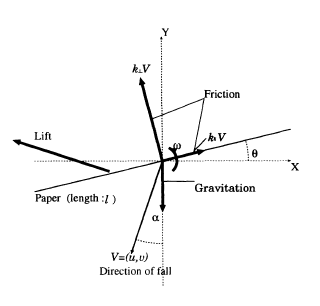
\includegraphics[width=0.7\textwidth]{FBD.png}
\caption{\label{fig:Leaf_diagram}Schematic showing the forces acting on the leaf.\cite{tanabe1994behavior}
}
\end{figure}
\noindent Figure \ref{fig:Leaf_diagram} shows a schematic of the forces acting on the leaf.
\\
\\
The differential equations can be solved using the fourth order Runge-Kutta Method. The initial conditions are all chosen to be zero, except the initial condition $\theta = 1$. The dynamics and motion of the leaf can be investigated by plotting phase-portraits in the u-v plane and the motion visualised by plotting the trajectory of the center of mass in the x-y plane with the length and angle of the leaf plotted at slight intervals.
\\
\\
\noindent The model considers $\theta$ in the range $\frac{-\pi}{2}<\theta<=\frac{\pi}{2}$, this causes a discontinuity in the value of theta when it increases beyond $\frac{\pi}{2}$ or falls below $\frac{-\pi}{2}$. This can be seen in Figure \ref{fig:Theta}, for this Figure the parameters had values $f=100,k_{\perp}=4.84,g=9.81,l=1,\rho=0.1$.

\begin{figure}[H]
\centering
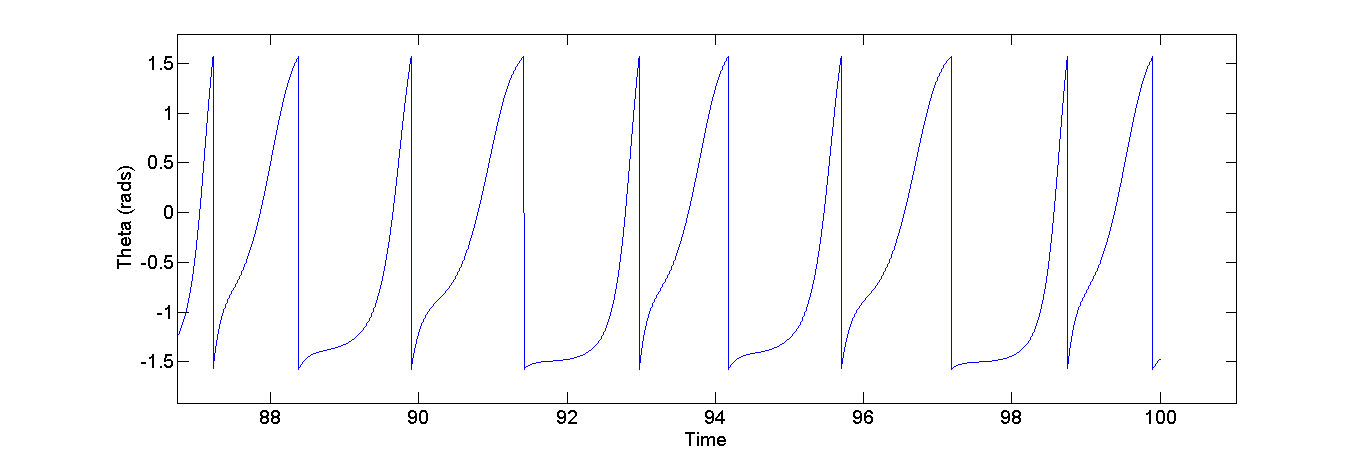
\includegraphics[width=0.7\textwidth]{Theta_discon.png}
\caption{\label{fig:Theta}Plot showing the angle of the leaf with time.
}
\end{figure}
\noindent As Figure \ref{fig:Theta} shows the value of $\theta$ falls from $\frac{\pi}{2}$ to a value near $\frac{-\pi}{2}$ instantly. This corresponds to the leaf crossing the y axis in the vertical position as it rotates. Another discontinuity will be experienced due to the $\pm$ signs in equations \ref{eq:motion_eqns}.



%% -- Continue here with the derivation of the equations. 

%% -- After derivation talk about method to solve equations, fourth order rk method (I think). 

%% -- Talk about discontinuity caused by +- sign and the limits put on theta